\documentclass[12pt]{scrartcl}

\usepackage[utf8]{inputenc}
\usepackage[IL2]{fontenc}
\usepackage[czech]{babel}
\usepackage{graphicx}
\usepackage{hyperref}
\usepackage{amsmath}
\usepackage[]{algorithm2e}
\usepackage{enumitem}
\usepackage{gensymb}

\subject{Západočeská univerzita v\nobreakspace Plzni\\Fakulta aplikovaných věd\\KIV/KPG}
\author{Pavel Zelenka\\A16B0176P\\zelenkap@students.zcu.cz}
\date{\today}
\title{Fraktály}

\begin{document}
\maketitle
\pagenumbering{gobble}
\newpage
\pagenumbering{arabic}
\newpage
\section{Zadání}
	
\paragraph{}
Zadáním úkolu je vytvoření nového programu nebo rozšíření programu ze cvičení, tak aby vykresloval fraktály, které nebyly na cvičení.

\section{Analýza problému}

\paragraph{}
\textbf{Fraktál} je\nobreakspace seběpodobný útvar, to znamená, že lze pozorovat stále opakující\nobreakspace se tvar. Mezi známe fraktály patří Sierpińského koberec, Sierpińského trojúhelník či křivka vyplňující prostor. V této práci se budu zabývat fraktály zvanými \textbf{Hexaflake}, \textbf{Sierpińského šestiúhelník}, \textbf{T-Square} a \textbf{Hilbertovou křivkou} vyplňující prostor. 

\subsection{Hexaflake a Sierpińského šestiúhelník}
Hexaflake je iterativně konstruovaný fraktál skládající se ze šestiúhelníků. V nulté počáteční iteraci existuje jeden šestiúhelník, který se po první iteraci rozdělí na 7 menších šestiúhelníků, které jsou uvnitř plochy původního šestiúhelníku. Každou další iteraci se každý šestiúhelník znovu rozdělí na 7 menších. Celkový počet šestiúhelníků je tedy $7^{n-1}$. Strana každého nového šestiúhelníků odpovídá $\frac{1}{3}$ velikosti strany předchozího šestiúhelníku.

Sierpińského šestiúhelník se implementuje obdobně s rozdílem, že se šestiúhelník rozděluje jen na 6 menších šestiúhelníků. Velikost strany zůstává stejná jako u Hexaflake, ale vypustí se prostřední šestiúhelník, tedy střed šestiúhelníku není v další iteraci vyplněn.

\subsection{Hilbertova křivka}
Hilbertova křivka lze implementovat iterativním způsobem, kdy se bude využívat binární reprezentace indexů bodů. Algortmus bude v cyklu provádět bitový posun a budou se zjišťovat vždy poslední 2 bity, dle kterých se bude měnit pozice.

\subsection{T-square}
T-square je iterativně konstruovaný fraktál skládající se ze čtverců. V nulté počáteční iteraci existuje jeden čtverec. V první iteraci vzniknou 4 nové čtverce o poloviční velikosti strany, každý z těchto čtverců bude mít střed na jedné z hran čtverce z předchozí iterace.

\section{Popis řešení}

\paragraph{}
Vykreslování probíhá ve\nobreakspace třídě \emph{Drawing}. Algortitmy fraktálů\nobreakspace se nacházejí v balíčku \emph{fractal}.

\subsection{Hexaflake}
Hexaflake je reprezentován třídou \emph{Hexaflake.java}, v metodě \emph{draw()} se provede výpočet středu okna a umístí se do tohoto místa počáteční bod. Velikost strany počátečního šestiúhelníku je pevně daná na $1/3$ šířky nebo výšky okna, dle menšího rozměru. Dle požadovaného počtu iterací se určí počet šestiúhelníků po poslední iteraci, tento údaj slouží pro duhové barvy.
\paragraph{}
Metoda \emph{calculateHexagon(double hw, double hh, double side)} provede výpočet hran šestiúhelníku.
\paragraph{}
\begin{algorithm}[H]
	\KwIn{šířka\_okna, výška\_okna, strana, strany}
	první\_bod = null\;
	předchozí\_bod = null\;
	\For{int i = 0; i < 6; i++} {
		x\_souřadnice = šířka\_okna$/2$ + strana + cos($i \cdot 2 \cdot pi / 6$)\;
		y\_souřadnice = výška\_okna$/2$ + strana + sin($i \cdot 2 \cdot pi / 6$)\;
		\eIf{předchozí\_bod != null} {
			nový\_bod = bod se souřadnicemi x\_souřadnice a y\_souřadnice\;
			strany[i-1] = úsečka mezi body předchozí\_bod a nový\_bod\;
			\If{i == 5}{
				strany[i] = úsečka mezi body nový\_bod a první\_bod\;			
			}
		} {
			první\_bod = nový\_bod\;
		}
		předchozí\_bod = nový\_bod\;
	}
	\caption{Vytvoření šestiúhelníku}
\end{algorithm}
\paragraph{}
Vykreslování a iterace probíhá v metodě \emph{drawHexagon(Point center, double side, int iteraction, int max)}. Metoda má jako parametry bod ve středu šestiúhelníku, velikost strany, pořadí současné iterace a celkový počet iterací.
\newpage
\subsection{Hilbertova křivka}
\paragraph{}
V práci je implementován algoritmus, který index bodu Hilbertovy křivky převádí do kartézské soustavy souřadnic bez použití rekurze. Algoritmus předpokládá, že bod s indexem $0$ je na pozici $[0,0]$. V první iteraci existují právě 4 body a počáteční křivka je pevně daná.

\paragraph{}
Pozice následujících bodů se dopočítávají podle indexu. Poslední 2 bity označují umístění bodu v rámci čtveřice bodů (tj.\nobreakspace tvar křivky v první iteraci), následující dvojice bitů označuje umístění předešlé čtveřice bodů v rámci šestnáctice bodů (tj.\nobreakspace křivka v druhé iteraci).

\begin{figure}[!ht]
	\centering
	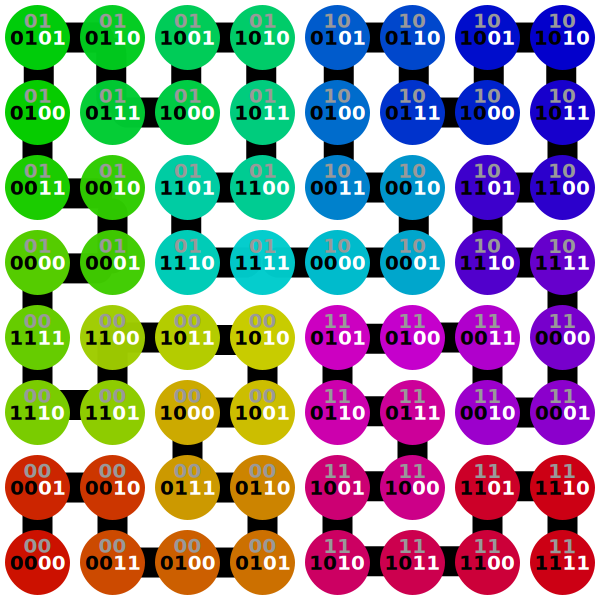
\includegraphics[width=0.6\textwidth,natwidth=1,natheight=1]{hilbert.pdf}
	\caption{Indexy bodů v třetí iteraci}
\end{figure}

\newpage
\section{Uživatelská dokumentace}

\paragraph{}
Spuštění aplikace se\nobreakspace provede souborem \texttt{Fractal.jar}, který se nachází ve složce \emph{App}. Po spuštění je nutné vybrat v dolním panelu křivku. Iterace se provede kliknutím na libovolné místo ve vykreslovací oblasti.

\begin{figure}[!ht]
	\centering
	\includegraphics[width=0.85\textwidth,natwidth=1,natheight=1]{app_gui.pdf}
	\caption{Okno aplikace}
\end{figure}

\newpage
\section{Závěr}
\paragraph{}
U aplikace není úplně vyřešeno omezení na určitý počet iterací fraktálu a proto u vyšší iterace může dojít ke zpomalení počítače či k vyčerpání dostupné paměti a pádu aplikace. Každá třída reprezentující fraktál má nastavený strop počtu iterací, ovšem problém je závislý  i na dalších faktorech a nepodařilo se mi jej spolehlivě vyřešit.


\section{Reference}

Hexagon – Wolfram MathWorld. [online].\\ Dostupné z: \href{http://mathworld.wolfram.com/Hexagon.html}{en.wikipedia.org/wiki/Hexaflake}
\\
Hexaflake – Wikipedia. [online].\\ Dostupné z: \href{https://en.wikipedia.org/wiki/Hexaflake}{en.wikipedia.org/wiki/Hexaflake}
\\
Iterative algorithm for drawing Hilbert curve – Marcin Chwedczuk. [online].\\ Dostupné z: \href{https://marcin-chwedczuk.github.io/iterative-algorithm-for-drawing-hilbert-curve}{marcin-chwedczuk.github.io/iterative-algorithm-for-drawing-hilbert-curve}

\end{document}
